\documentclass[11pt]{article}

%We want to be wider
\usepackage{a4wide}

% Input encoding
\usepackage[utf8]{inputenc}
\usepackage{eurosym}

\usepackage{caption}
\usepackage{subcaption}

%Syntax Highlighting
\usepackage{listings}

\usepackage{color}
\definecolor{gray}{rgb}{0.4,0.4,0.4}
\definecolor{darkblue}{rgb}{0.0,0.0,0.6}
\definecolor{cyan}{rgb}{0.0,0.6,0.6}

\lstset{
  basicstyle=\ttfamily,
  columns=fullflexible,
  showstringspaces=false,
  commentstyle=\color{gray}\upshape
}

\lstdefinelanguage{XML}
{
  morestring=[b]",
  morestring=[s]{>}{<},
  morecomment=[s]{<?}{?>},
  stringstyle=\color{black},
  identifierstyle=\color{darkblue},
  keywordstyle=\color{cyan},
  morekeywords={xmlns,version,type}% list your attributes here
}
% Math packages
\usepackage{amsfonts}
\usepackage{amssymb}
\usepackage{amsmath}

\usepackage{tikz,stex,amstext}

%Add some color
\usepackage{xcolor}

% WE want colored links instead of ugly boxes
\usepackage[colorlinks=true]{hyperref}
\usepackage{url}

% Ednotes
\usepackage[show]{ed}

% We're actually using a units package, so we might also search this document.
\usepackage{siunitx}
\sisetup{load-configurations = abbreviations}

% BibTex
\usepackage{cite}

\title{Semantic Search For Quantity Expressions\\ \vspace{2 mm} Bachelor Thesis DRAFT\ednote{Remove draft status}}
\author{Tom Wiesing\\Supervisor: Michael Kohlhase\\Co-supervisor: Tobias Preusser\\Jacobs University, Bremen, Germany}

\date{\today}

\usetikzlibrary{shapes,arrows,mmt}

\begin{document}

%Title Page
\maketitle

%The abstract
\begin{abstract}

  \noindent In this paper we want to give an approach to Semantic Search for Quantity Expressions.

  A Quantity Expression is an expression that represents a quantity such as $25 \frac{\text{m}}{\text{s}}$. Different Quantity Expressions can represent the same quantity, for example the expression can also be refered to by $90 \frac{\text{km}}{\text{h}}$. In this case we are only using metric units, however using different units can become a problem when having to convert between them constantly.

  In a Semantic Search Engine for Quantity Expressions we want to be able to search for quantities independent of their representations. The implementation we have designed is very modular. We use a meta-mathematical formalisation for the unit system. This brings the advantage of being easily extensible with new units. Because of the modularity, the spotting of Quantity Expressions within documents is taken on in \cite{thesis:sherko}.

  Despite this modularity, our implementation has some problems, one of them being that we can not translate between \textit{Celsius} and \textit{Kelvin}. Nonetheless, if expanded and improved properly, this implementation has potential to solve the problem of different units entirely.

\end{abstract}

\newpage

\tableofcontents

\newpage

\section{Introduction}

\subsection{The Problem Of Units}

Units are everywhere. We encounter units and quantity expressions in everyday life wherever we go. When driving on the road we see a speed limits on signs (for example $30 \frac{\text{km}}{s}$). When we go shopping there are different shoe sizes. When we buy something, we pay a currency of $30 \text{\euro}$. Everything is being quantified. This is also the case in science papers. Many, if not all, papers have 1 or more quantity expressions in them. Approximatly 1\% of all letters in scienficic papers belong to a quantity expression\ednote{Verify this}.

This in itself is not a problem. The problem occurs when different units are used to describe the same quantity. In most of the world, the metric system is used to describe most quantities. However some countries still use other units which often leads to accidents.

These different units sometimes make it very difficult to talk about Quantity Expressions. One notable example for this is the \textit{Mars Climate Orbiter} which was destroyed in 1999 when it entered the atmosphere of Mars because it received the non-standard units of \textit{pound-seconds} instead of the expected \textit{newton-seconds}\cite{nasa:mcor}.

\subsection{State Of The Art: Unit Converters And The SI System}

Out of convenience new units ones are constantly being invented. Hence there are many hundred units that already exist. Just converting between them is easy, googleing ``unit converter'' reveals about 12000000 results\ednote{Perhaps quote the google result page here?}. Even Google itself has implemented a unit converter into its search engine.

However, all of these tools have a problem. They only convert units directly, meaning they require the user to enter the original units and desired units. This reuires the user to identity that there is a problem with units in the first place.

There is no tool which directly incorperates this translation of units into search results. Such a tool should find quantities independently of which units they are expressed in. It would make search efforts much easier, as fewer user input is required. It would no longer be required for the user to recognise that there is a problem.

In addition to this problem unit converters are usually very restricted in the units they support. They commonly store translation formulae for any pair of units to convert between. Hence they are difficult to extend with new units.

Their superficial handling of units usually does not take the underlying meaning, the semantics, into accoun On the other hand, The SI specification \cite{sispec} provides a very good insight into how units can be handled. It is precisely defined what each unit means and what kind of quantities can be expressed. It is a very formal approach. This approach does not take into account that it is sometimes less practical to user general units instead of specfic ones. Furthermore notation of SI units is not always exact\ednote{More explanation}.

Neither this very formal nor the previous approach with unit converters can be efficiently used to solve the problem.

\subsection{Our Approach: A Semantic Quantity Expression Search}

That is why we want to build a search engine that unifies these approaches. It should be capable to find occurrences of quantity expressions within documents, no matter of their representation. For this we need several components: (1) an extensible system flexible enough to convert between units when needed, (2) a so-called spotter that finds occurrences of quantity expressions within documents, (3) a search algorithm that can take a quantity expression from the user and find equivalent ones in the results from the spotter and (4) a front-end that allows the user to enter a quantity expression and receive the results.

For (1) we want to use a meta-mathematical theories approach. With the help of MMT this allows us to build an extendible unit system. This uses a concept of a theory graph in which units are related via so-called views and imports. These can be used to translate between them. Additionally, we can define a new unit and easily link it to any of the ones which have been defined previously. Point (2) will be taken on by Stiv Sherko in a seperate effort \cite{proposal:sharko}. The spotter finds quantity expressions inside documents which can almost directly be used by our system. For our search algorithm (3) we use a simple trick: When finding units, we normalise them to a normal form. This normal form is then used to efficiently index the harvest delivered from the previous step. Finally for (4) we built a frontend which allows the user to enter quantity expressions. It is deployed at \ednote{Link the deploy site here. }.

\ednote{Make a system diagram and refer to it here. }

\subsection{Overview}

This thesis is organised as follows: In section \ref{sec:mathoverview} we start by giving an introduction to mathematical theory modeling. We proceed in section \ref{sec:strucqe} to talk about how quantity expressions can be formalised and in section \ref{sec:mqes} we apply these insights in order to start building in our search engine. In section \ref{sec:pit} we present the implementation in detail by describing how a search query is processed and how it is presented to the end user. After discussing the limits of this implementation as well as future work in section \ref{sec:future} we conclude in section \ref{sec:conclusion}.


\newpage

\section{The Structure Of Mathematics: Theories, Views And Imports}
\label{sec:mathoverview}

Before we start looking at Quantity Expressions and how to build a search engine for them, we want to give an introduction to meta-mathematical structure. We will use this knowledge later to build a better search engine.

To model mathematics we need a proper logical foundation. For this we use the \textit{LF Logical Framework} \cite{hhp93lf}. LF provides a typed logic, that is a logic in which each object has a so-called type. It also allow to construct functions as types via the $\rightarrow$ constructor.

Next we can take a look at the concept of theories.

\subsection{Modeling Mathematics With The Help Of Theories}

Theories, in this sense, are simply sets of symbols. Each of the symbols can optionally have a type and a definition. Within each theory, we can then use these symbols to write down terms (or expressions) within this theory. Types and definitions of these symbols are terms themselves\footnote{They are not terms over the same theory however. }. As a simple example of this, let us consider the theory of semigroups as seen in Figure \ref{fig:semigroup}.

\begin{figure}[h]
  \begin{center}
    \begin{tabular}{|l c l|}
      \hline
      \textsf{Semigroup} & &\\\hline
      $G$ & $:$ & $ \mathsf{type}$\\
      $\circ$ & $:$ & $ G \rightarrow G \rightarrow G$\\
      $ \mathsf{assoc}$& $:$ & $ \text{ded}\left( \forall x \in G . \forall y \in G . \forall z \in G . (x\circ y)\circ z=x\circ (y\circ z) \right)$\\\hline
    \end{tabular}
  \end{center}

  \caption{The theory of semigroups. }
  \label{fig:semigroup}
\end{figure}


In this theory, we define 3 symbols: $G$, $\circ$ and $\scriptstyle \mathsf{assoc}$. In the first line we define a type $G$. Next we define a function $\circ$ that takes 2 terms of type $G$ and returns another term of type $G$. We could also denote this function by $G \times G \rightarrow G$ but LF does not provide the $\times$ symbol. Hence we just use the equivalent notation $G \rightarrow G \rightarrow G$. In the last line, we make the statement that associativity holds. This is achieved via the \textit{ded} (short for deduction) symbol. When a statement (such as associativity formulation in this case) is passed to it, it asserts that the statement is provable by returning a proof for it. Thus it is commonly used for axiomes.

\subsection{Extending Theories Using imports}

Sometimes we want to extend theories without having to define everything again. For example, we want to say that a Monoid is a semi-group along with an identity element. In the semi-group example above, we have also used terms from other theories to define $G$ as a type.

We can model this concept by using imports. An import from one theory into another makes symbols of the imported theory available in the target theory. In Figure \ref{fig:monoid} we can easily define a monoid.

\begin{figure}[h]
  \begin{center}
    \begin{tabular}{|l c l|}
      \hline
      \textsf{Monoid} & &\\\hline
      $ \mathsf{import \ Semigroup}$ &&\\
      \hline
      $e$ & $:$ & $G$\\
      $ \mathsf{id}$& $:$ & $ \text{ded}\left( \forall x : G . x\circ e = e \circ x = x\right)$\\\hline
    \end{tabular}
  \end{center}
  \caption{The Theory Of Monoids Which Imports The Theory Of Semigroups As Defined In Figure \ref{fig:semigroup}. }
  \label{fig:monoid}
\end{figure}


\subsection{Views As Truth-Preserving Mappings Between Theories}

However imports are not the only way how theories can be related. If we have 2 theories, we sometimes want to have a map between them. In addition to the theory of monoids above we define the theory of non-negative integers in Figure \ref{fig:nnintegers}.

\begin{figure}[h]
  \begin{center}
    \begin{tabular}{|l c l|}
      \hline
      \textsf{Non-negative integers} & &\\\hline
      $\mathbb{Z}^{+}_{0}$ & $:$ & $\mathsf{type}$\\

      $0$ & $:$ & $\mathbb{Z}^{+}_{0}$\\

      $+$ & $:$ & $ \mathbb{Z}^{+}_{0} \rightarrow \mathbb{Z}^{+}_{0} \rightarrow \mathbb{Z}^{+}_{0}$\\

      $\mathsf{assoc}$& $:$ & $ \text{ded}\left( \forall x : \mathbb{Z}^{+}_{0} . \forall y : \mathbb{Z}^{+}_{0} . \forall z : \mathbb{Z}^{+}_{0} . (x\circ y)\circ z=x\circ (y\circ z) \right)$\\

      $\mathsf{id}$& $:$ & $ \text{ded}\left( \forall x \in \mathbb{Z}^{+}_{0} . x + 0 = 0 + x = x\right)$\\\hline
    \end{tabular}
  \end{center}
  \caption{The theory of non-negative integers. }
  \label{fig:nnintegers}
\end{figure}


A map from the theory of monoids to the theory of positive integers should map all symbols from the theory of monoids to symbols from the theory of positive integers. Furthermore, such a map should be truth preserving, i. e. if I write down a true statement as a term over the theory of monoids and translate this term, it should still be true  in the theory of positive integers. Such a mapping is called a \textit{View} from the theory of monoids to the theory of Positive integers. Such a view $\phi$ could look as follows:

\[
  \phi=\left\{\begin{array}{l}
  G \mapsto \mathbb{Z}^{+}_{0}\\
  e \mapsto 0\\
  \circ \mapsto +\\
  \mathsf{assoc} \mapsto \mathsf{assoc}\\
  \mathsf{id} \mapsto \mathsf{id}
  \end{array}\right\}
\]

If we take a closer look at this view, we notice that we also have to map the imported symbols. This is needed so that we can translate any term or statement in theory of monoids to a term or statment into the theory of non-negative integers.

\subsection{Building Theory Graphs}

We have seen in the examples above that we can model mathematics with the help of theories, views and imports. To make this structure even more obvious, we can represent it in a graph, a so-called theory graph. We consider the theories as vertices of such a graph and the views and imports as edges. An example can be found in Figure \ref{fig:groups_full}.

\def\thmo#1#2{\mathsf{#1}\colon\kern-.15em{#2}}
\providecommand\myxscale{3.9}
\providecommand\myyscale{2.2}
\providecommand\myfontsize{\footnotesize}

\begin{figure}[h]
  \begin{center}
    \begin{tikzpicture}[xscale=\myxscale,yscale=\myyscale]\myfontsize
      \node[thy] (sg) at (1,-1) {
        \begin{tabular}{l}
          \textsf{Semigroup}\\\hline
          $G,\circ$\\\hline
          $\scriptstyle x\circ y\in G$ \\\hline
          $\scriptstyle \mathsf{assoc}: (x\circ y)\circ z=x\circ (y\circ z)$
        \end{tabular}
      };
      \node[thy] (m) at (1,0) {
        \begin{tabular}{l}
          \textsf{Monoid}\\\hline
          $e$\\\hline
          $\scriptstyle e\circ x=x$
        \end{tabular}
      };
      \node[thy] (g) at (1,1) {
        \begin{tabular}{l}
          \textsf{Group}\\\hline
          $i := \scriptstyle\lambda x.\tau y. x\circ y=e$\\\hline
          $\scriptstyle\forall x:G.\exists y:G.x\circ y=e$
        \end{tabular}
      };
      \node[thy] (cg) at (1,2) {
        \begin{tabular}{l}
          \textsf{Commutative Group}\\\hline
          \\\hline
          $\scriptstyle \mathsf{comm} : x\circ y=y\circ x$
        \end{tabular}
      };



      \node[thy] (N) at (-1,-1) {
        \begin{tabular}{l}
          \textsf{Natural Numbers}\\\hline
          $\mathbb{N},s,0$\\\hline
          $\scriptstyle P1$,\ldots $\scriptstyle P5$
        \end{tabular}
      };
      \node[thy] (Np) at (-1,0) {
        \begin{tabular}{l}
          \textsf{Natural Numbers with Plus}\\\hline
          $+$\\\hline
          $\scriptstyle n+0=n$,\\
          $\scriptstyle n+s(m)=s(n+m)$
        \end{tabular}
      };
      \node[thy] (Nt) at (-1,1) {
        \begin{tabular}{l}
          \textsf{Natural Numbers with Multiplication}\\\hline
          $\cdot$\\\hline
          $\scriptstyle n\cdot1=n$,\\
          $\scriptstyle n\cdot s(m)=n\cdot m+n$
        \end{tabular}
      };
      \node[thy] (ia) at (-1,2) {
        \begin{tabular}{l}
          \textsf{Integer Arithmetics}\\\hline
          $-$\\
          $\mathbb{Z} := \mathbb{N}\cup-\mathbb{N}$\\\hline
          $\scriptstyle-0=0$
        \end{tabular}
      };

      %Right side
      \draw[include] (sg) -- (m);
      \draw[include] (m) -- node[left] (mg) {$\mathsf{g}$} (g);
      \draw[include] (g) -- (cg);

      %Left side
      \draw[include] (N) -- (Np);
      \draw[include] (Np) -- (Nt);
      \draw[include] (Nt) -- (ia);

      %Links
      \draw[view] (m) -- node[above] {$
      \thmo{f}{
      \left\{\begin{array}{l}
        G\mapsto\mathbb{N}\\
        \circ\mapsto +\\
        e\mapsto 0
      \end{array}\right\}
      }$
      } (Np);
      \draw[view] (cg) -- node[above] {$\thmo{h}{
      \left\{\begin{array}{l}
        i\mapsto -\\
        \mathsf{g}\mapsto\mathsf{f}
      \end{array}\right\}
      }$} (ia);
    \end{tikzpicture}
  \end{center}

  \caption{A Simple Theory Graph. Imports Are Represented As Solid Edges And Views As Wavey Edges. The Mappings Of The Views Are Given Explicitly. We Omit The Complete Definitions Of The Peano Axiomes For The Natural Numbers. }
  \label{fig:groups_full}
\end{figure}


\subsection{Using MMT To Write Down Terms And Theories}

MMT is a \textbf{M}odule system for \textbf{M}athematical \textbf{T}heories \cite{RabKoh:WSMSML13}. With the help of MMT we can represent theories, views and imports in \textit{.mmt} files. It is easy to write these files and anyone without programming knowledge can easily extend existing ones. The objects defined in these files can then be used via an API to write down terms and transform these using definitions and views.

This furthermore allows us to easily model an extensible system for units for use within a search engine. We will come back to this later in section \ref{sec:meq_model}.


\newpage

\section{The Structure Of Quantity Expressions}
\label{sec:strucqe}

The first step in developing a good search engine for Quantity Expressions is to take a closer look at Quantity Expressions.

When looking at Quantity Expressions, we need to distinuish between two perspectives, a notational one (i. e. the way they are written down) and a semantic one (i. e. what they mean).

\subsection{Compositional Behaviour Of Quantity Expressions}
Let us start by the behaviour of the notation. For this purpose let us take a look at:
\[x = 25\ \frac{\text{m}}{\text{s}}\]
We notice that $x$ consists of 2 parts, a scalar ($25$) and a scalar-free $\frac{\text{m}}{\text{s}}$ one. Furthermore, the unit consists of two primitive units $m$ and $s$. Since they divide one another, we can conclude that $x$ describes a velocity.

In general, the \textit{unit component} is not always scalar free. While $m$ and $s$ certainly do not contain scalars, this is no longer the case in the following example:
\[y = \frac{\text{L}}{100\ \text{km}}\]
We could certainly call $y$ a \textit{unit}. It consists of 2 sub-expressions, $\text{L}$ and $100\ \text{km}$. The first one is a primitive unit and the second one a multiplication of a number and the unit $\text{km}$. This, first of all, leads us to define the concept of a \textit{primitive unit} as a simple Quantity that is not a Number.

Abstracting from the examples above, we can now considder the semantics of Quantity Expressions. It makes sense to define Quantity Expressions as one of the following 6 cases:
\begin{enumerate}
  \item A \textit{primitive unit}, such as \textit{Meter}.
  \item The \textit{Product} of a Quantity Expression with a scalar, such as $5 \text{Meter}$
  \item The \textit{Quotient} of a Quantity Expression by a (non-zero) scalar\footnote{Strictly speaking, this is equivalent to the case above. For simplicity we define it anyways. }.
  \item The Multiplication $\cdot{}$ which takes 2 existing quantity expression and generates a new one, for example $\cdot \left(100, \text{m} \right) = 100\ \text{m}$
  \item The division / which again takes 2 quantity expressions and generates a new one, for example $\text{/} (\text{m}, \text{s}) = \frac{\text{m}}{\text{s}}$
  \item The addition of two quantity expressions \footnote{This is also not strictly needed, but can become useful later on when we want to translate between different units. }
\end{enumerate}

This allows us to easily generate Quantity Expressions (like the examples $x$ and $y$ from above) starting at the primitive units m, s, L and km.

\subsection{Dimensions Of Quantity Expressions}
Next let us briefly examine the dimensions of Quantity Expressions. The dimension of a Quantity Expression is the type of quantity it expresses. For example $5\ \text{m}$ describes some length. According to the International System of Units \cite{sispec} there are seven basic dimensions:
\begin{enumerate}
  \item length
  \item mass
  \item time
  \item electric current
  \item temperature
  \item luminous intensity
  \item amount of substance.
\end{enumerate}

In addition to these we found that there are commonly two other dimensions: The \textit{count} dimension (used for counting of objects) and the \textit{none} dimension for dimensionless quantities.

Similar to the compositional behaviour of Quantity Expressions, dimensions can be multiplied and divided. In this the \textit{count} dimension behaves like a multiplicative identity element.

Unlike Quantity Expressions however dimensions can not be multiplied with numbers. Furthermore, when multiplying to Quantity Expressions of dimensions $a$ and $b$ their resulting dimension is $a \cdot{} b$, the product of the dimensions. The same goes for division. In this regard the dimension of a quantity expression behaves like a type.

\subsection{A Mathematical Theory Of Quantity Expressions}
\label{sec:qeform}

The realisation that dimensions are types of quantity expressions leads us to our first formalisation of Quantity Expressions. We first define a theory of dimensions in Figure \ref{fig:dimensions} and then import it to define a theory of Quantity Expressions in Figure \ref{fig:QE}.

\begin{figure}[h]
  \begin{center}
    \begin{tabular}{|l c l|}
      \hline
      \textsf{Dimension} & &\\\hline
      $\mathsf{dimension}$ & $:$ & $ \mathsf{type}$\\

      $\mathsf{none}$ & $:$ & $ \mathsf{dimension}$\\
      $\mathsf{count}$ & $:$ & $ \mathsf{dimension}$\\
      $\mathsf{length}$ & $:$ & $ \mathsf{dimension}$\\
      $\mathsf{mass}$ & $:$ & $ \mathsf{dimension}$\\
      $\mathsf{time}$ & $:$ & $ \mathsf{dimension}$\\
      $\mathsf{current}$ & $:$ & $ \mathsf{dimension}$\\
      $\mathsf{temperature}$ & $:$ & $ \mathsf{dimension}$\\
      $\mathsf{luminous}$ & $:$ & $ \mathsf{dimension}$\\
      $\mathsf{amount}$ & $:$ & $ \mathsf{dimension}$\\

      $\cdot{}$ & $:$ & $ \mathsf{dimension} \rightarrow \mathsf{dimension} \rightarrow \mathsf{dimension}$\\
      $/$ & $:$ & $ \mathsf{dimension} \rightarrow \mathsf{dimension} \rightarrow \mathsf{dimension}$\\\hline
    \end{tabular}
  \end{center}
  \caption{A Formalization Of The Theory Of Dimensions. }
  \label{fig:dimensions}
\end{figure}


\begin{figure}[h]
  \begin{center}
    \begin{tabular}{|l c l|}
      \hline
      \textsf{Quantity Expression} & &\\\hline
      $ \mathsf{import \ Dimension}$ &&\\
      $ \mathsf{import \ Number}$ &&\\
      \hline
      $\mathsf{QE}$ & $:$ & $ \mathsf{dimension} \rightarrow \mathsf{type}$\\
      $\mathsf{QENMul}$& $:$ & $ \forall x : \mathsf{dimension} . \mathsf{number} \rightarrow \mathsf{QE}\left( x\right) \rightarrow \mathsf{QE}\left( x\right)$\\
      $\mathsf{QENDiv}$& $:$ & $ \forall x : \mathsf{dimension} . \mathsf{QE}\left( x\right) \rightarrow \mathsf{number} \rightarrow \mathsf{QE}\left( x\right)$\\

      $\mathsf{QEMul}$& $:$ & $ \forall x : \mathsf{dimension} . \forall y : \mathsf{dimension} . \mathsf{QE}\left( x\right) \rightarrow \mathsf{QE}\left( y\right) \rightarrow \mathsf{QE} \left( \cdot{} \left(x, y\right) \right)  $\\
      $\mathsf{QEAdd}$& $:$ & $ \forall x : \mathsf{dimension} . \mathsf{QE}\left( x\right) \rightarrow \mathsf{QE}\left( x\right) \rightarrow \mathsf{QE} \left( x \right)  $\\
      $ \mathsf{QEDiv}$& $:$ & $ \forall x : \mathsf{dimension} . \forall y : \mathsf{dimension} . \mathsf{QE}\left( x\right) \rightarrow \mathsf{QE}\left( y\right) \rightarrow \mathsf{QE} \left( \backslash \left(x, y\right) \right)  $\\\hline
    \end{tabular}
  \end{center}

  \caption{The Chosen Formalization Of The Theory Of Quantity Expressions. }
  \label{fig:QE}
\end{figure}


Figure \ref{fig:dimensions} defines the 9 basic dimensions and then dimension compositon via multiplication and division. Then we move on in Figure \ref{fig:QE} to define quantity expressions. Each quantity expression has a dimension (via the \textit{QE} constant). This allows us to define basic units (which we will actually do in the next Figure). With the \textit{QENMul} and \textit{QENDiv} symbols we can multiply and divide quantity expressions by numbers (for this case we actually need to import some theory of numbers to allow us actually write this down as a Term). Then we define multiplication and division of quantity expressions in such a way that dimensions multiply and divide appropriatly.

Now we need to introduce some basic units. Let us start by just defining \textit{Meter} in Figure \ref{fig:meter}. We can now write a term in this theory that expresses any number of meters.

\begin{figure}[h]
  \begin{center}
    \begin{tabular}{|l c l|}
      \hline
      \textsf{Meter} & &\\\hline
      $ \mathsf{import \ Quantity Expression}$ &&\\
      \hline
      $\mathsf{Meter}$ & $:$ & $ \mathsf{QE} \left( \mathsf{length} \right)$\\\hline
    \end{tabular}
  \end{center}

  \caption{A Theory Defining The Primitive Unit Meter. }
  \label{fig:meter}
\end{figure}


\subsection{Transforming Quantity Expressions From One Form Into Another}
\label{sec:qeconv}

This provides a basis for a unit system. Let us furthermore define a few more units of non-metric lengths. In Figure \ref{fig:nonsilength} we show a few non-si units. Here we first define thoug as a quanity expression of length and then one-by-one define more units in terms of the previous one.
\begin{figure}[h]
  \begin{center}
    \begin{tabular}{|l c l|}
      \hline
      \textsf{Meter} & &\\\hline
      $ \mathsf{import \ Quantity Expression}$ &&\\
      \hline
      $\mathsf{Thou}$ & $:$ & $ \mathsf{QE}\left( \mathsf{length} \right)$\\
      $\mathsf{Foot}$ & $:$ & $ \mathsf{QE}\left( \mathsf{length} \right) = \mathsf{QEMul} \left( \mathsf{QENum} \left(1000 \right), \mathsf{Thou} \right)$\\
      $\mathsf{Yard}$ & $:$ & $ \mathsf{QE}\left( \mathsf{length} \right) = \mathsf{QEMul} \left( \mathsf{QENum} \left(3 \right), \mathsf{Foot} \right)$\\
      $\mathsf{Chain}$ & $:$ & $ \mathsf{QE}\left( \mathsf{length} \right) = \mathsf{QEMul} \left( \mathsf{QENum} \left(22 \right), \mathsf{Yard} \right)$\\
      $\mathsf{Furlong}$ & $:$ & $ \mathsf{QE}\left( \mathsf{length} \right) = \mathsf{QEMul} \left( \mathsf{QENum} \left(10 \right), \mathsf{Chain} \right)$\\
      $\mathsf{Mile}$ & $:$ & $ \mathsf{QE}\left( \mathsf{length} \right) = \mathsf{QEMul} \left( \mathsf{QENum} \left(8 \right), \mathsf{Furlong} \right)$\\
      \hline
    \end{tabular}
  \end{center}

  \caption{A theory of some non-SI units of length. }
  \label{fig:nonsilength}
\end{figure}


We now want to relate quantity expressions with units from the \textit{Meter} theory to units from the \textit{Non SI Lengths} theory. It is known that $1 \mathsf{Thou} = 0.0000254 \mathsf{Meter}$. This can be easily expressed with a view $\psi$ between these two theories:

\[
\psi = \left\{\begin{array}{l}
  \mathsf{Thou} \mapsto \mathsf{QENMul} \left( 0.0000254, \mathsf{Meter} \right)
\end{array}\right\}
\]

Even though the view just maps the symbol \textit{Thou} to some Term in the Meter theory, we can also use it to transform any other term from the Thou Theory. Since all units are defined in terms of the previous one, we can just expand all definitions to get an expression containing only numbers and the unit \textit{Thou}. Then we can use the view as normal to get a Quantity Expression in the \textit{Meter} theory.


\newpage

\section{Making Quantity Expressions searchable}
Having investigated the structure of quantity expression in the previous section, we can now define a meta-mathmatical theory of quantity expressions as our next step towards a search engine.

\subsection{A meta-mathmatical formalisation of quantity expressions}
\label{sec:meq_model}

\subsection{Normalisation of Quantity Expressions}
* describe normalisation algorithm, 2 steps

\subsection{Serialising Quantity Expressions to XML}
* W3C RFC, find it again

%\label{sec:mws:tg}

%The theories and their relations can be represented as a graph, called a theory graph. In Figure \ref{graph1} we can see a simple example of a theory graph.

%\usetikzlibrary{shapes,arrows,mmt}
\def\thmo#1#2{\mathsf{#1}\colon\kern-.15em{#2}}
\providecommand\myxscale{3.9}
\providecommand\myyscale{2.2}
\providecommand\myfontsize{\footnotesize}

\begin{figure}[h]
\begin{tikzpicture}[xscale=\myxscale,yscale=\myyscale]\myfontsize
  \node[thy] (sg) at (1,-1) {
    \begin{tabular}{l}
      \textsf{Semigroup}\\\hline
      $G,\circ$\\\hline
      $\scriptstyle x\circ y\in G$ \\\hline
      $\scriptstyle \mathsf{assoc}: (x\circ y)\circ z=x\circ (y\circ z)$
    \end{tabular}
  };
  \node[thy] (m) at (1,0) {
    \begin{tabular}{l}
      \textsf{Monoid}\\\hline
      $e$\\\hline
      $\scriptstyle e\circ x=x$
    \end{tabular}
  };
  \node[thy] (g) at (1,1) {
    \begin{tabular}{l}
      \textsf{Group}\\\hline
      $i := \scriptstyle\lambda x.\tau y. x\circ y=e$\\\hline
      $\scriptstyle\forall x:G.\exists y:G.x\circ y=e$
    \end{tabular}
  };
  \node[thy] (cg) at (1,2) {
    \begin{tabular}{l}
      \textsf{Commutative Group}\\\hline
      \\\hline
      $\scriptstyle \mathsf{comm} : x\circ y=y\circ x$
    \end{tabular}
  };



  \node[thy] (N) at (-1,-1) {
    \begin{tabular}{l}
      \textsf{Natural Numbers}\\\hline
      $\mathbb{N},s,0$\\\hline
      $\scriptstyle P1$,\ldots $\scriptstyle P5$
    \end{tabular}
  };
  \node[thy] (Np) at (-1,0) {
    \begin{tabular}{l}
      \textsf{Natural Numbers with Plus}\\\hline
      $+$\\\hline
      $\scriptstyle n+0=n$,\\
      $\scriptstyle n+s(m)=s(n+m)$
    \end{tabular}
  };
  \node[thy] (Nt) at (-1,1) {
    \begin{tabular}{l}
      \textsf{Natural Numbers with Multiplication}\\\hline
      $\cdot$\\\hline
      $\scriptstyle n\cdot1=n$,\\
      $\scriptstyle n\cdot s(m)=n\cdot m+n$
    \end{tabular}
  };
  \node[thy] (ia) at (-1,2) {
    \begin{tabular}{l}
      \textsf{Integer Arithmetics}\\\hline
      $-$\\
      $\mathbb{Z} := \mathbb{N}\cup-\mathbb{N}$\\\hline
      $\scriptstyle-0=0$
    \end{tabular}
  };


  \node (psi) at (0,-.5) {
    $\psi=\left\{\begin{array}{l}
    G\mapsto\mathbb{N}\\
    \circ\mapsto +\\
    e\mapsto 0\end{array}\right\}$
  };

  \node (phi) at (0,1.7) {
    $\phi=\left\{\begin{array}{l}
    i\mapsto -\\
    \mathsf{g}\mapsto\mathsf{f}
    \end{array}\right\}$
  };

  %Right side
  \draw[include] (sg) -- (m);
  \draw[include] (m) -- node[left] (mg) {$\mathsf{g}$} (g);
  \draw[include] (g) -- (cg);

  %Left side
  \draw[include] (N) -- (Np);
  \draw[include] (Np) -- (Nt);
  \draw[include] (Nt) -- (ia);

  %Links
  \draw[view] (m) -- node[above] {$\thmo{f}\psi$} (Np);
  \draw[view] (cg) -- node[above] {$\thmo{h}{\phi}$} (ia);
\end{tikzpicture}

\caption{A simple theory graph. Imports are represented as solid edges and views as dashed edges. }
\label{graph1}
\end{figure}
 \ednote{Explain the mappings somewhere}

%Every theory and every constant in MMT has a (globally unique) URI, called the MMT URI. It can be constructed via a triple $\left( G,M,S \right)$ where $G$ is a document URI, $M$ is a module name within this document and $S$ is the name of a constant \cite{RabKoh:WSMSML13}. We then seperate these components via a ? to get a URI of the form $G?M?S$. Because every theorem in MMT is only a symbol declaration it can also be represented via a URI. As explained above, if two theories are related via a view or import, theorems can be translated along this relation.

%Sometimes it is useful not to write down a theorem explicitly, but only give an existing theorem and translate this along a view or import. The MMT URI of this induced theorem can then be given using the view. This URI contains enough information for MMT to generate the theorem in explicit form\cite{IanKohProd:rassmk14}.

%In an MWS Harvest we exploit this property of induced theorems. We have several represented theorems, the forumlae in the corpus, and many more induced theorems, other equivalent representations of these formulae. With the help of MMT, the MMT Harvest is built by representing all theses theories (forumlae) explictly.

%Applying this principle to quantity expressions, we can consider different units as different theories and different quantity expressions different theorems belonging to their respective unit theories. The unit conversions can then be represented via views. The information on how to translate from one unit to another will be contained within the view. If we know all formulae in a corpus we can then generate an MWS Harvest that contains all the representations.



%As mentioned above, MathWebSearch is a search engine for forumlae and key phrases\ednote{Work in TEMA Search}. MWS consists of 3 main components as well as a frontend\footnote{The frontend is not part of MWS directly but rather built on top of the REST API, more on this later. }\cite{KohPro:MWSmanual}.

%The backend consists of 3 main components,
%\begin{enumerate}
%  \item a crawler,
%  \item a core system and
%  \item a public REST API.
%\end{enumerate}

%The crawler, as its name suggests, crawls corpera for forumlae. For each corpus MWS uses, a seperate crawler has to be implemented. The crawled formulae are passed to the core system and indexed in an MWS Harvest. The core system is also responsible for parsing queries and sending results back to the REST API. This is done by searching the harvest only. In order to make a semantic search for quantity expressions we will adapt this crawler to find and harvest quantity expression instead.

%Because MWS is semantics-aware, the harvest can not only contain the exact formulars that are found in the original corpus but also all versions that are quivalent to it. These are generated with the help of MMT and theory graphs, see sections \ref{sec:mws:mmt} and \ref{sec:mws:tg}.

%The frontend for MathWebSearch, which is not part of MWS itself but running client-side in a web browser, is written in HTML5, CSS and JavaScript. It accesses the REST backend and depends on MathML support to render Mathematics. When the client enters a query to search for, the \LaTeX{}ml daemon \cite{latexml-daemon} is used to transform the query into content MathML. Next, the client renders the MathML (to show the formular the user is searching for) and then sends the query off to the MWS API. Upon receiving results, the client renders them and links to the original documents. \ednote{ScreenShot of MWS} \ednote{Write about Query Expansion vs Index Expansion}

%There are several implementations of frontends and crawlers as well as extensions of MathWebSearch. One particular implementation is capable of crawling the arXMLiv corpus, which contains approximatly 750.000 documents. A list of demos can be found at \cite{URL:MWSDemo}.


\newpage

\section{The Implementation: The Search Process}
\label{sec:pit}

Now that we have discussed all the theoretical components of the search engine, it is time to move on to the actual implementation. In this section we describe in detail how a search query is processed and how it is presented to the end user.

\subsection{Entering A Query}

As to give an overview of what exactly happens during a typical search, we will show what happens during a normal search process. From the user perspective, everything happens inside a web browser. When the user visits the demo page \cite{self:sqesdemo}, they are presented with a frontend as shown in Figure \ref{fig:frontmain}.

\begin{figure}[h]
  \begin{center}
    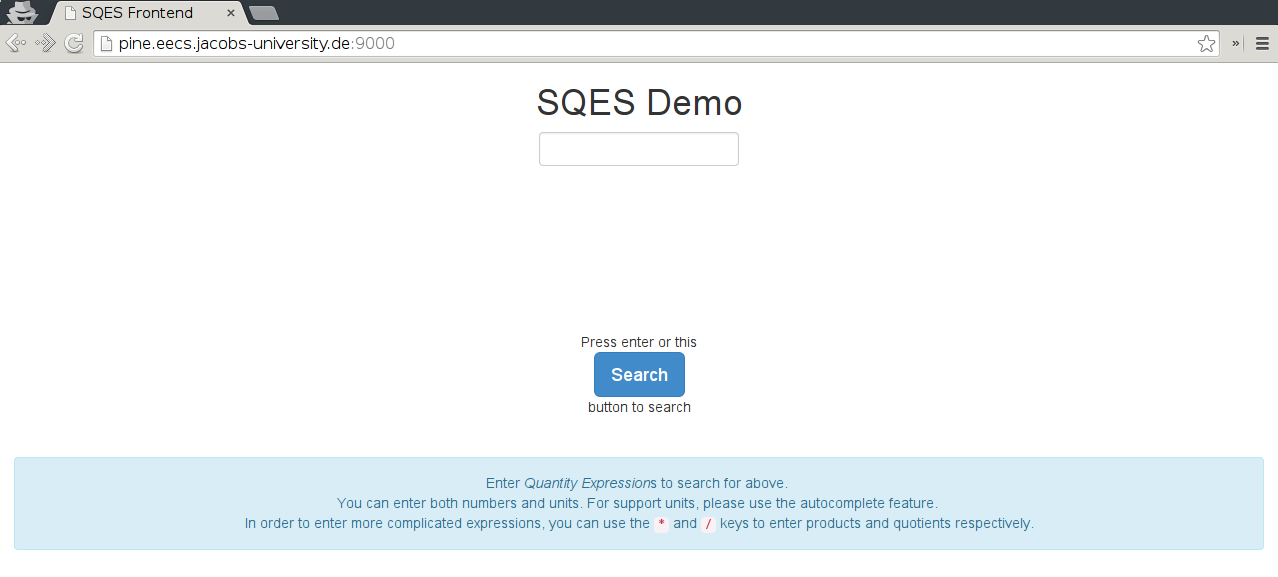
\includegraphics[width=100mm]{img/screen1.png}
  \end{center}
  \caption{The main page of the frontend. }
  \label{fig:frontmain}
\end{figure}

Because the frontend is running inside a Webbrowser it is written using HTML, CSS and JavaScript. Furthermore it uses the frameworks jQuery \cite{lib:jquery} and Bootstrap \cite{lib:bootstrap}. As seen in the figure, the main components are a text field to enter a quantity expression as well as a search button.

With the text field it is easily possible to enter composed quantity expression.

When searching for a certain unit it is neccessary to tell the backend which \textit{unit theory} this unit comes from. In order to make this easier, the GUI has an autocompletion feature. It is only required to enter the name of the unit itself and the possible theories this unit can come from will be suggested automatically.

Apart from entering a simple unit it is possible for the user to compose quantity expressions by multiplication and division. If the keys ``*'' and ``/'' are pressed, the text field splits into two different fields. In each of them another quantity expression can be entered.

In order to facilitate entering division and multiplication by numbers, it is also possible to enter numbers into these fields. With this input unit it is also possible to enter all the quantity expressions as described by the formalism above. In Figure \ref{fig:frontauto} the process of entering the query $42 \frac{\text{Furlong}}{\text{Fortnight}}$ is shown.

\begin{figure}
  \centering
  \begin{subfigure}[b]{0.9\textwidth}
          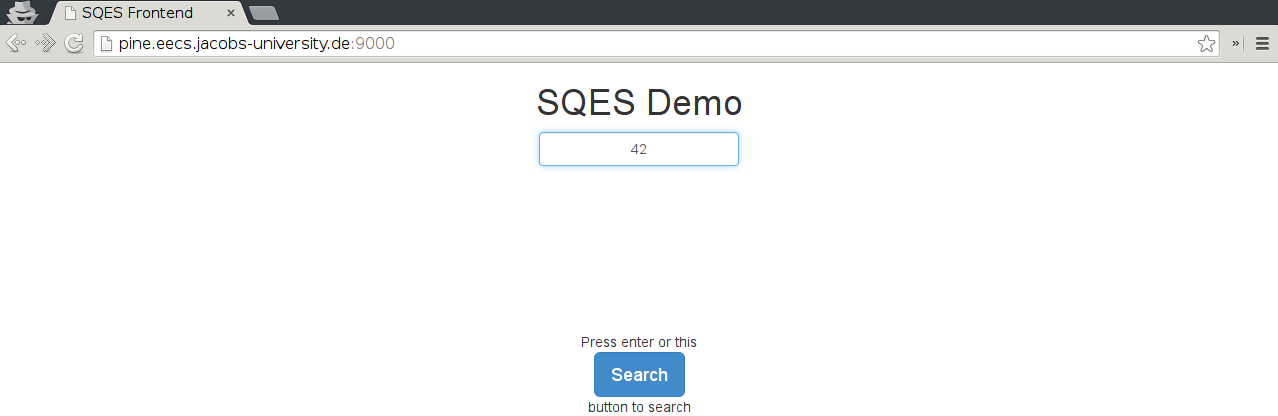
\includegraphics[width=\textwidth]{img/enter1}
          \caption{Entering a number}
          \label{fig:frontauto1}
  \end{subfigure}
  \\
  \begin{subfigure}[b]{0.9\textwidth}
          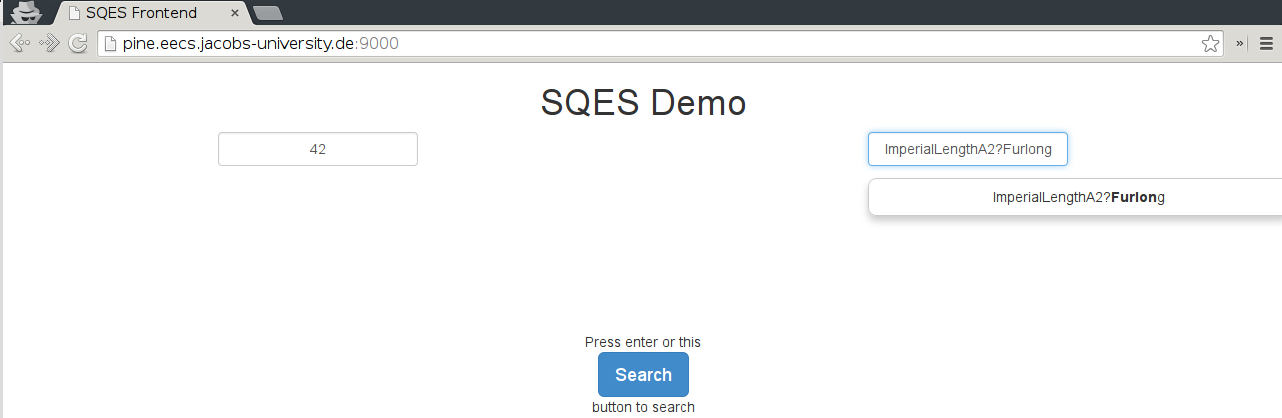
\includegraphics[width=\textwidth]{img/enter2}
          \caption{Entering and autocompleting the unit \textit{Furlong}}
          \label{fig:frontauto2}
  \end{subfigure}
  \\
  \begin{subfigure}[b]{0.9\textwidth}
          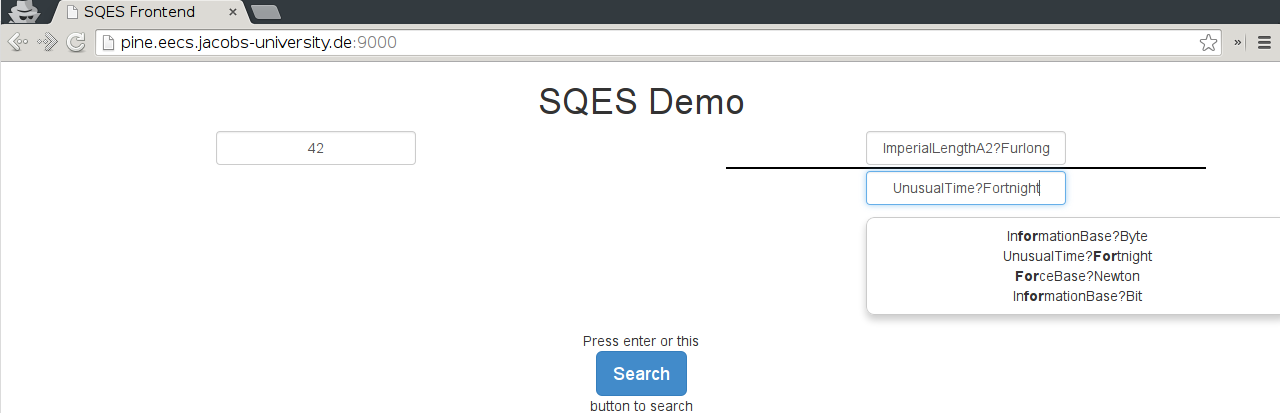
\includegraphics[width=\textwidth]{img/enter3}
          \caption{Entering the final component. }
          \label{fig:frontauto3}
  \end{subfigure}
  \caption{Process of entering the quantity expression $42 \frac{\text{Furlong}}{\text{Fortnight}}$ into the frontend. }
  \label{fig:frontauto}
\end{figure}

\subsection{Preparing The Backend}

After the quantity expression has been entered, the search can be started by pressing the \textit{Search} button or hitting the \textit{Enter} key. The query inputted into the text field is then serialised to XML as shown in Section \ref{sec:xml}. This XML is then sent to the backend.

The backend is written in Scala and exposes its functionality via HTTP. Before the backend is ready to receive queries, it has to normalise the quantity expressions found by the Spotter. These queries are also provided in XML form. This XML is parsed and deserialised into an internal data structure.

Next we want to normalise these quantity expressions using the algorithm described in Section \ref{sec:norm}. In order to achieve this the backend first parses the MMT theories and views and builds up a theory graph. Next, it normalises all units found inside the unit graph and caches these normal forms in memory.

We can then use the forms to quickly normalise all the quantity expression found inside the harvests. The normalised forms are then used to store them in an appropriate structure on disk. In this structure all equivalent quantity expressions are stored inside the same folder. This allows very quick access to all quantity expressions in preparation for processing a query.

\subsection{Processing A Typical Query}

Upon receiving the query, the backend deserialises and normalises the XML as it did for all the harvests. Since the normal forms of each \textit{basic unit} are still cached inside memory, this process is very quick. Because the normal forms are already cached on disk, the process of finding equivalent quantity expressions can be efficiently done. As described above, all equivalent quantity expressions are in the same folder. The backend now just reads all the quantity expressions stored inside the folder the query falls in. This delivers all equivalent quantity expressions and can be sent back the frontend.

Because all the normal forms are simply stored on disk inside a folder it is easily possible to add more quantity expressions to an existing harvest. This is even possible during query timee. For this reason the implementation of the search engine has two seperate modes, a \textit{harvest} mode and a \textit{query} mode which allow preprocessing of harvests and actual querying. Since the first mode does not require network interaction, only the query mode has an actual HTTP interface.

\subsection{Presenting The Results}

After the results have been received by the backend they are displayed to the user. An example can be found in Figure \ref{fig:frontres} \ednote{Make this picture}.

\begin{figure}
  \caption{The result page when searching for $100$ Meters. }
  \label{fig:frontres}
\end{figure}


\newpage

\section{Future work}
\subsection{Extension of the theory graph of units}

\subsection{Integration with MathWebSearch}

%Most of the components will inherit from the existing MathWebSearch system. Some of the work packages, like the theory graph, will be easy to complete whereas others, like the unit system, need more work.

%A view between theories of units is enough to translate between them. In practice however, because we want to use units in several components of the system, it is insufficient to just look at the theory graph views. We will need to develop a unit system that can efficiently handle units as well as translations.

%To translate between units we could use simple translation formulae such has $x \text{K} = x + 273.15 ^\circ{C} $. However because we want to support composite units (such as meters per second $\frac{\text{m}}{\text{s}}$) as well, this can cause problems. When translating between 2 composite units, this can easily cause rounding errors. In particular, when an author gives an approximation of a quantity expression in a document, they might round differently depending on the units used. Thuse we might want to search for a range of values instead. This has recently been implemented as an extension to MathWebSearch\cite{MWS:Ranges}. It remains to be seen how exactly these ranges should be used and handled in the front end.

%Apart from translating, we will also need to enter the units in the frontend and pass them to the API. The representation we choose for units when translating should also be flexible enough so that they can be entered easily. While it is trivial to design an interface where a single unit can be entered, it is non-trivial when we want to recognise composite units as well. Furthermore units with (si-)prefixes (such as kilo or mega) can either be recognised seperatly or as part of the unit (multipling directly into the value of the quantity expression). There are several input formats that can be used: AsciiMath, \LaTeX{} and MathML, to name only a few.


\newpage

%BIBLIOGRAPHY
\bibliography{kwarc,thesis}{}
\bibliographystyle{alpha} %plainURI?
\end{document}
